
% JuliaCon proceedings template
\documentclass{juliacon}
\setcounter{page}{1}

%%---- definition of custom commands
\newcommand{\abs}[1]{\left|#1\right|}
\newcommand{\vb}{\boldsymbol}
%%----

\begin{document}

% **************GENERATED FILE, DO NOT EDIT**************

\title{My JuliaCon proceeding}

\author[1]{1st author}
\author[1, 2]{2nd author}
\author[2]{3rd author}
\affil[1]{University}
\affil[2]{National Lab}

\keywords{Julia, Optimization, Game theory, Compiler}

\hypersetup{
pdftitle = {My JuliaCon proceeding},
pdfsubject = {JuliaCon 2022 Proceedings},
pdfauthor = {1st author, 2nd author, 3rd author},
pdfkeywords = {Julia, Optimization, Game theory, Compiler},
}



\maketitle

\section{Summary}
% from the JOSS docs:
% The paper should include a summary describing the high-level functionality and purpose of the software for a diverse, non-specialist audience.

%--- What is Peridynamics? ---%
\texttt{Peridynamics.jl} is an open source Julia \cite{bezanson2017julia} implementation of the nonlocal continuum mechanics formulation by Silling (ref?).
In peridynamics, a body is described by material points and, based on interactions between them, internal force densities are calculated. 
The equation of motion reads
\begin{equation}
    \varrho \, \vb{\ddot{u}}(\vb{X},t) = \vb{b}^{\mathrm{int}}(\vb{X},t) + \vb{b}^{\mathrm{ext}}(\vb{X},t) \qquad \forall \vb{X} \in \mathcal{B}_0, \; t \geq 0 \; ,
\end{equation} 
with the mass density $\varrho$, the point acceleration vector $\vb{\ddot{u}}$, and the point force density vectors $\vb{b}^{\mathrm{int}}$ and $\vb{b}^{\mathrm{ext}}$. 
In the original bond-based formulation (BB), the internal force density is calculated by
\begin{equation}
    \vb{b}^{\mathrm{int}}(\vb{X},t) = \int_\mathcal{H} \vb{f} \; \mathrm{d}V' \; ,
\end{equation}
with the \emph{pairwise force function} $\vb{f}$, which is evaluated for each material point $\vb{X}^i$ and depends on the deformation of the bonds to each point in its neighborhood $\mathcal{H}$.
These point families contain each point within a distance $\delta$, also called horizon.

To overcome the restrictions of the BB formulation with only one determinable material parameter, the state-based formulation was established.
Here not only the bonds to neighboring material points, but also the states of neighboring points influence the internal force density $\vb{b}^{\mathrm{int}}$ of each material point.
The equation reads
\begin{equation}
    \vb{b}^{\mathrm{int}} (\vb{X},t) = \int_\mathcal{H} \vb{t} - \vb{t}' \; \mathrm{d}V' \; ,
\end{equation}
with the force vector states $\vb{t}=\vb{t}(\vb{\Delta X}, t)$ and $\vb{t}'=\vb{t}(-\vb{\Delta X}, t)$.

%--- What is the high-level functionality of Peridynamics.jl? ---%
The \texttt{Peridynamics.jl} package enables users to perform peridynamic simulations.

\begin{figure}
\centerline{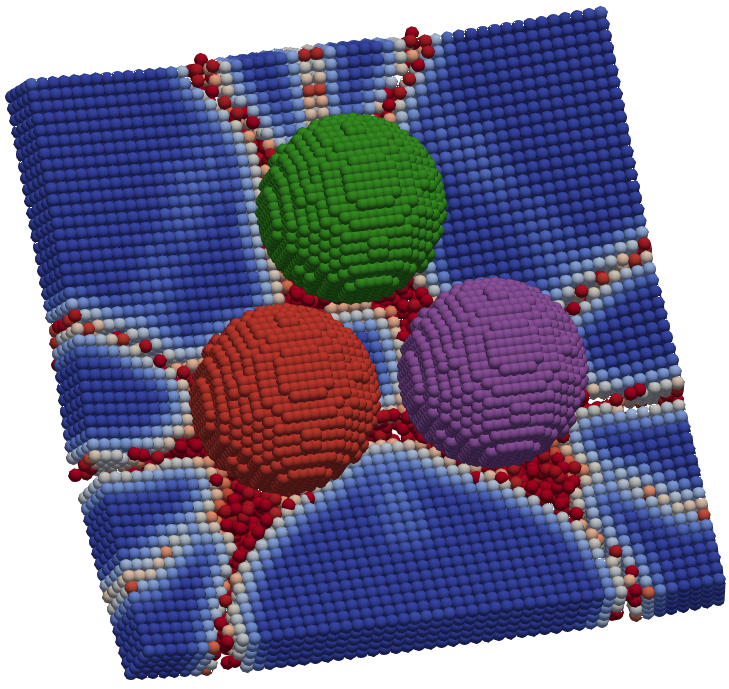
\includegraphics[width=0.8\linewidth]{logo.png}}
\caption{High-velocity contact simulation of three spheres crashing into a rectangular panel; logo of Peridynamics.jl}
\label{fig:logo}
\end{figure}

\begin{figure}
\centerline{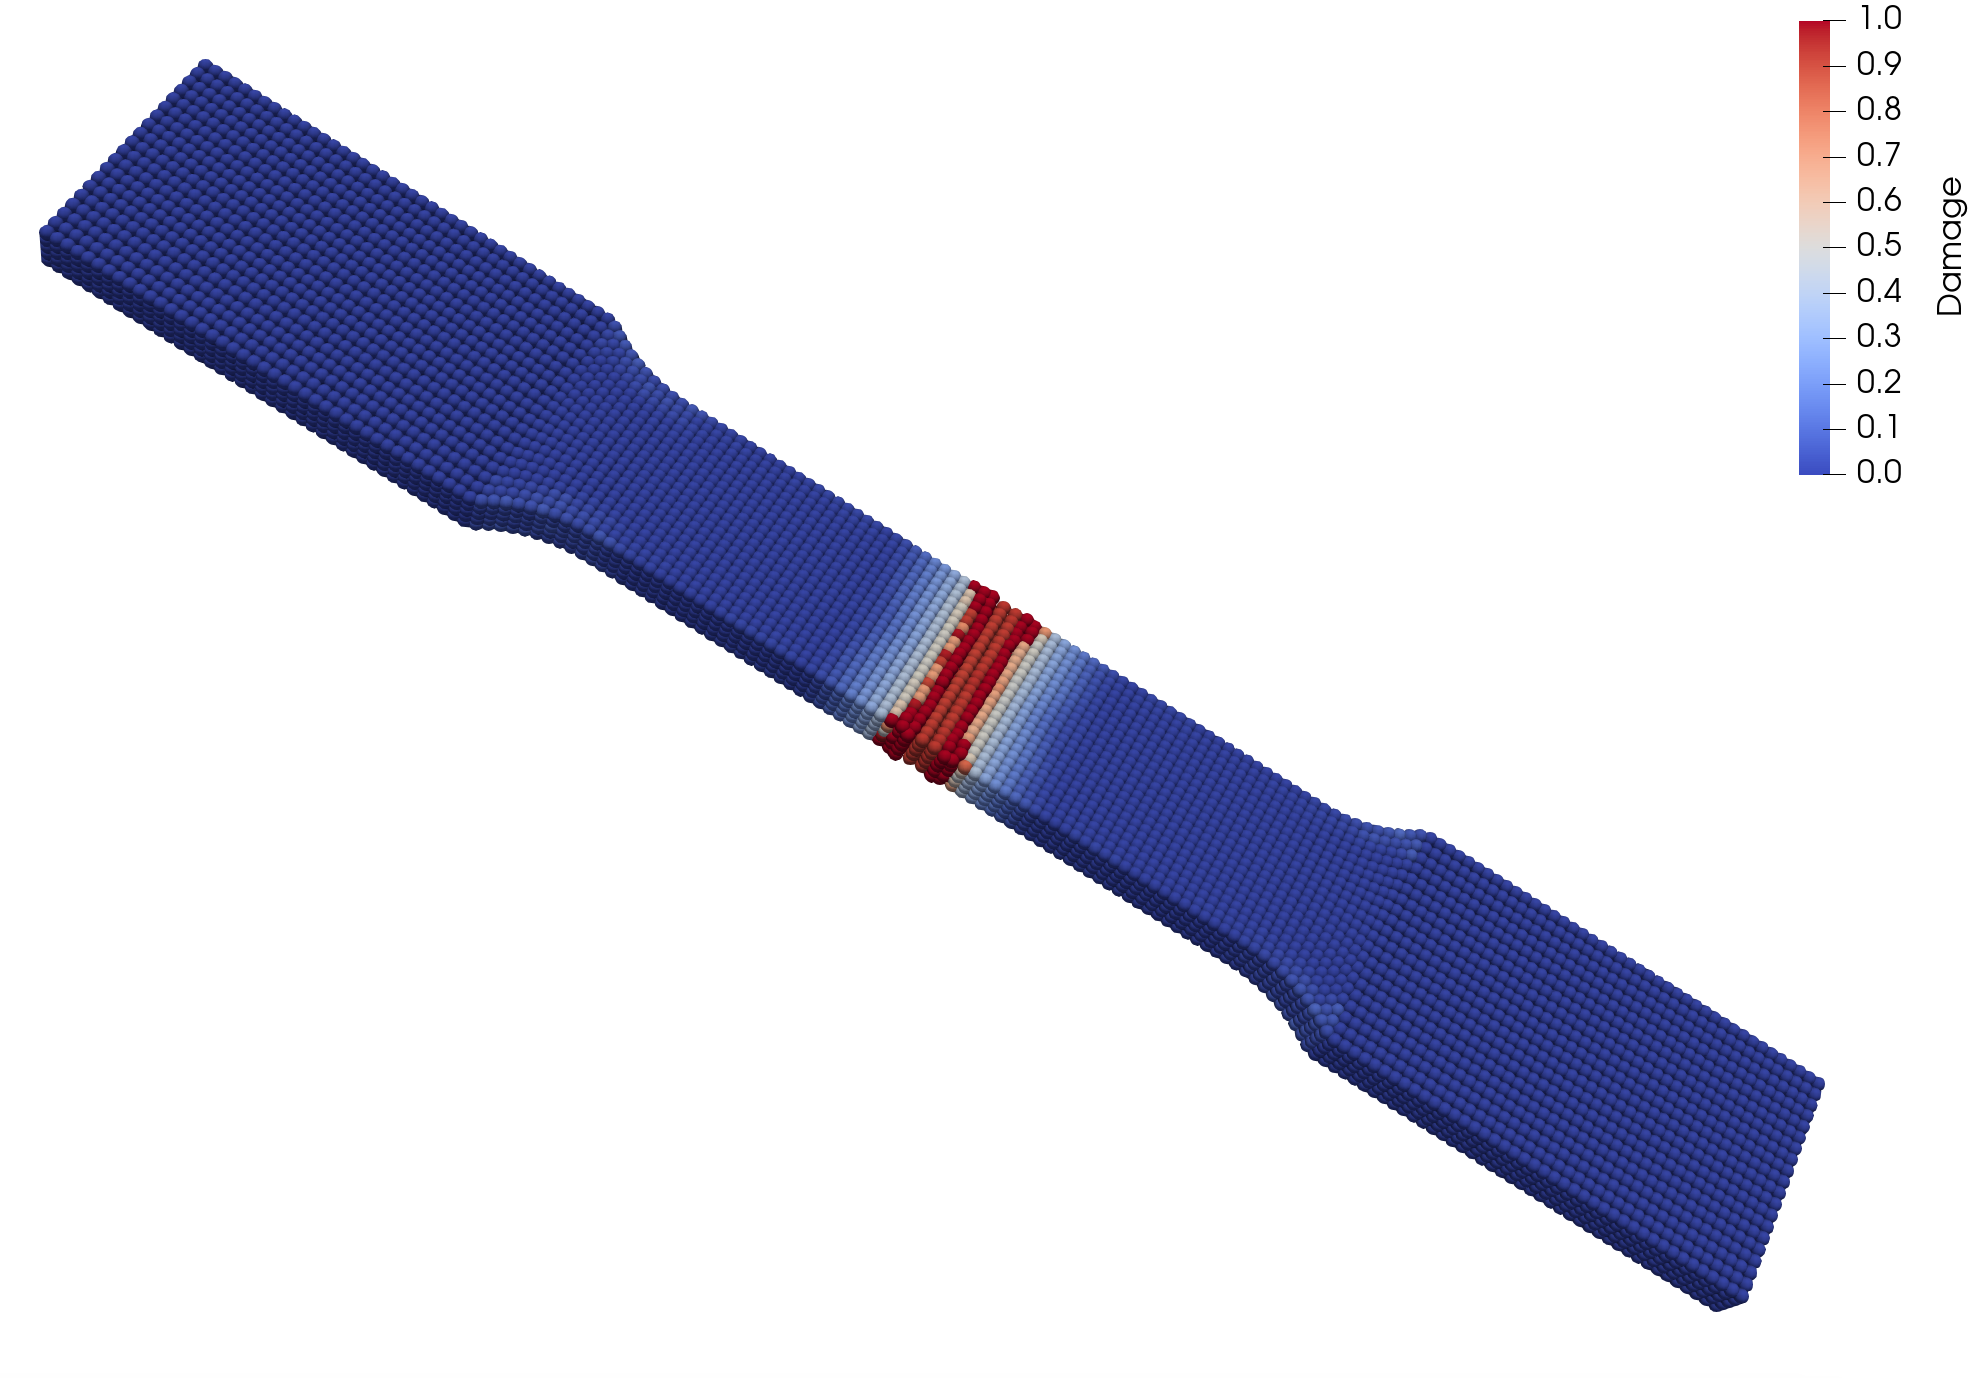
\includegraphics[width=0.8\linewidth]{tensile_test.png}}
\caption{Fracture simulation of tensile tension test with a crack propagating in the middle of the specimen}
\label{fig:tensiletest}
\end{figure}

\section{Statement of need}
% from the JOSS docs:
% The paper should include a Statement of need section that clearly illustrates the research purpose of the software and places it in the context of related work.

%--- Place the package in the context of related work
The package was already used in numerous publications, e.g. \cite{Friebertshaeuser2022PAMM,Friebertshaeuser2022AIMS,Partmann2023IJF,Partmann2024AAM,Partmann2024PAMM,Tornquist2022PAMM}.

%--- What is the research purpose of Peridynamics.jl?


\section{Acknowledgments}
The authors gratefully acknowledge the support of the Deutsche Forschungsgemeinschaft (DFG) in the project \mbox{WE~2525/15-1}.

The authors gratefully acknowledge the support and the supercomputing resources of the Paderborn Center for Parallel Computing (https://pc2.uni-paderborn.de).

% \vadjust{\vfill\pagebreak}

% **************GENERATED FILE, DO NOT EDIT**************

\bibliographystyle{juliacon}
\bibliography{ref.bib}


\end{document}

% Inspired by the International Journal of Computer Applications template
